\documentclass[12pt]{article}
\usepackage[margin=1in]{geometry}
\usepackage{float}
\usepackage{xcolor}

\usepackage{wrapfig}
\usepackage{amsmath, amsthm, amssymb, mathtools}
\usepackage{newpxtext, newpxmath}

\usepackage{physics}

\NewDocumentCommand{\R}{}{\mathbb{R}}

\usepackage{thmtools}

\RenewDocumentCommand{\qedsymbol}{}{$\blacksquare$}

\declaretheorem{theorem}
\declaretheorem{lemma}
\declaretheorem[style=definition]{definition}

\declaretheorem{example}
\declaretheorem[style=remark]{remark}

\usepackage{tikz}
\usepackage{tcolorbox}
\tcbuselibrary{skins}

% \tcolorboxenvironment{theorem}{
%     empty,
%     borderline west={2pt}{0pt}{black}
% }

% \tcolorboxenvironment{definition}{
%     empty,
%     borderline west={2pt}{0pt}{black}
% }

\usepackage[style=alphabetic]{biblatex}
\addbibresource{sources.bib}

\usepackage{hyperref}

\hypersetup{
    colorlinks,
    citecolor=blue,
    linkcolor=blue,
    filecolor=blue,      
    urlcolor=blue,
}

\title{The Graph Laplacian and Determining the Connectivity of Meshes}
\author{Eli Griffiths}
\date{November 2024}

\directlua{graph = require("graph")}
\directlua{examples = require("data")}

\begin{document}

\maketitle

\begin{abstract}
    Beyond traditional combinatoric approaches, we can analyze the properties of graphs using the eigenvalues and eigenvectors of their matrix representations. We first show that a given graph’s Laplacian matrix eigenvalues encodes the connectedness of the graph. We then use this fact to solve a problem of mesh connectedness in computational geometry through a natural dual correspondence between meshes and graphs.   
\end{abstract}

\section{Introduction}

\section{Background}

We first outline the basic structure of a graph and related definitions that will be used throughout the paper, following the formalism and notation from \cite{diestelGraphTheory2017}. We adopt the notation that $[S]^n$ is the set of all $n$-element sized subsets of $S$.

\begin{definition}[Graph Structure]
    A \textbf{graph} is a pair $G = (V, E)$ of sets where $E \subseteq [V]^2$. The elements of $V$ are \textbf{vertices} and the elements of $E$ are \textbf{edges}. A vertex $v$ is said to be \textbf{incident} to an edge $e$ if $v \in e$. Two vertices $v_1$ and $v_2$ are \textbf{neighbors} if $\qty{v_1, v_2} \in E$. We denote $\qty{v_1, v_2} \in E$ by $v_1 \sim v_2$. The \textbf{set of neighbors} of a vertex $v$ is denoted by $N(v) \coloneq \qty{w \in V : v \sim w}$. The \textbf{degree} of a vertex $v$ is $\deg(v) \coloneq |N(v)|$.
\end{definition}

\begin{remark}
    Edges importantly are defined here as two element sets and not as ordered pairs. This makes the graph \textit{undirected}. If the graph was to be directed (that is the edges were to be ordered pairs) the further results of this paper would not hold in general and would require more restrictions.
\end{remark}

For the purposes of this paper, we will assume that every graph has finitely many vertices (and hence finitely many edges). A way to visualize a finite graph is by representing vertices as points in the plane and edges as line segments between these points as seen in Figure \ref{fig:basic_graph}.

\begin{figure}[H]
    \centering
    \begin{tikzpicture}[
        vertex/.style={
            inner sep=2pt,
            circle,
            draw,
            fill=blue!20,
        },
        edge/.style={}
        ]
        \directlua{graph.graph_tikz(examples.example1)}
    \end{tikzpicture}   
    \caption{A graph with $7$ nodes and $15$ edges}
    \label{fig:basic_graph}
\end{figure}


\begin{definition}[Adjacency and Degree Matrix]
    The adjacency matrix $A_G$ and degree matrix $D_G$ of a finite graph $G$ with $n$ vertices are the $n \times n$ matrices such that
    \begin{align*}
        (A_G)_{ij} = \begin{cases}
            1 & v_i \sim v_j \\
            0 & \text{otherwise}
        \end{cases} & &
        (D_G)_{ij} = \begin{cases}
            \deg(v_i) & i = j \\
            0 & i \neq j
        \end{cases}
    \end{align*}
\end{definition}

\begin{align*}
    A_G =    
    \begin{bmatrix}
        \directlua{graph.adj_matrix(examples.example1)}
    \end{bmatrix} & &
    D_G = \begin{bmatrix}
        \directlua{graph.deg_matrix(examples.example1)}
    \end{bmatrix}
\end{align*}

An important observation is that the adjacency matrix is symmetric. That is because for any vertices $v_i$ and $v_j$ we have both $v_i \sim v_j$ and $v_j \sim v_i$ meaning $(A_G)_{ij} = (A_G)_{ji}$. Since the adjacency matrix is symmetric, we know that it must have an orthonormal basis of eigenvectors and corresponding set of eigenvalues. Since $A_G$ is symmetric for any graph $G$, it begs the question: what can we determine about a graph based on these eigenvalues and eigenvectors?

\section{A Graph's Spectra}

\begin{definition}[Laplace Matrix]
    The \textbf{Laplacian Matrix} of a graph $G$ is $L_G \coloneq D_G - A_G$. If $G$ is understood via context, we simply refer to it as $L$.
\end{definition}

\begin{theorem}
    Let $L$ be the laplacian matrix of a finite graph $G$ with $n$ vertices. Then for a given vector $x \in \R^n$,
    \[
        x^T L x = \sum_{v_i \sim v_j} (x_i - x_j)^2.
    \]
    We call $x^T L x$ the quadratic form of $L$.
\end{theorem}

\begin{proof}
    We can rewrite $x^T L x = x^T (D - A) x$ using the definition of the Laplacian matrix. Expanding out we get
    \[
        x^T L x = x^T D x - x^T A x
    .\]
    First consider the term $x^T D x$. By the definition of $D$, we know that $(D)_{ij} = \deg(v_i)$ when $i = j$ and $0$ otherwise. Therefore
    \[
        x^T D x = \sum_{i=1}^n \sum_{j=1}^n x_i (D)_{ij} x_j = \sum_{i=1}^n \deg(v_i) \cdot x_i^2
    .\]
    Consider some vertex $v \in V$. Then $\deg(v)$ is also the number of edges containing $v$. Therefore we can rewrite the previous sum as a sum over the edges,
    \[
        \sum_{i=1}^n \deg(v_i) \cdot x_i^2 = \sum_{v_i \sim v_j} x_i^2 + x_j^2
    .\]
    Now consider $x^T A x$. By the definition of $A$, we know that $(A)_{ij} = 1$ if $v_i \sim v_j$ and $0$ otherwise. Therefore
    \[
        x^T A x = \sum_{i=1}^n \sum_{j=1}^n x_i (A)_{ij} x_j = 2 \cdot\sum_{v_i \sim v_j} x_i x_j
    .\]
    Note the factor of $2$ is needed because summing over entries of $A$ double counts edges. We have then
    \[
        x^T L x = x^T D x - x^T A x = \sum_{v_i \sim v_j} \qty(x_i^2 - 2 x_i x_j + x_j^2) = \sum_{v_i \sim v_j} (x_i - x_j)^2
        .\qedhere
    \]
\end{proof}

\begin{lemma}
    A connected graph $G$ is connected if and only if the $0^\text{th}$ eigenvalue of $L_G$ has algebraic multiplicity $1$.
\end{lemma}

\begin{theorem}
    A graph $G$ has $k$ connected components if and only if the $0^\text{th}$ eigenvalue of $L_G$ has algebraic multiplicity $k$.
\end{theorem}

\section{Application to Computational Geometry}
\begin{wrapfigure}[7]{r}{0.3\textwidth}
    \centering\vspace{-2cm}
    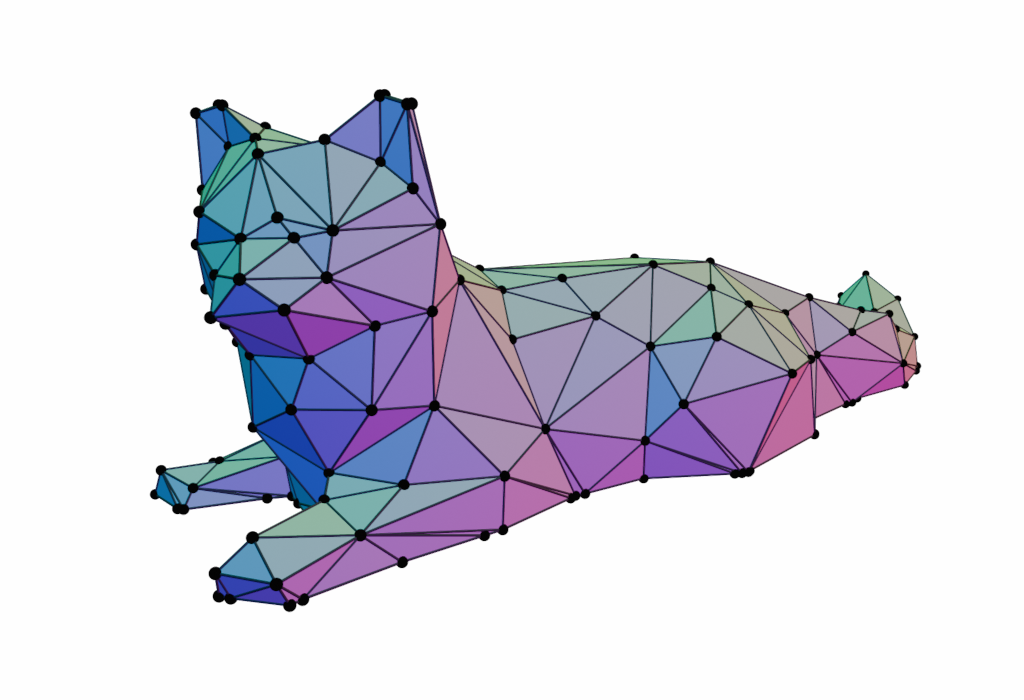
\includegraphics[width=0.5\pagewidth]{figures/cat.png}
\end{wrapfigure}

In computer graphics, modeling, simulation, etc. we often want a representation of some real world geometry that we can perform computations on. A common way to of doing so is via a mesh. Consider the example mesh of a cat to the right. From some basic observations, the mesh appears to be comprised of points connected by segments/edges which outline faces. We formalize these observations in Definition \ref{def:tri_mesh}.

\newpage
\begin{definition}[Triangular Mesh]
    \label{def:tri_mesh}
    A \textbf{triangular mesh} is a triple $K = (V, E, F)$ such that
    \begin{itemize}
        \item $V \subseteq \R^3$ is a finite set representing the vertices
        \item $E \subseteq [V]^2$ is a set representing non-intersecting edges
        \item $F \subseteq [E]^3$ is the set of faces such that for any $f = \qty{e_1, e_2, e_3} \in F$, we have $e_1 \cap e_2 = \qty{v_1}$, $e_2 \cap e_3 = \qty{v_2}$, and $e_3 \cap e_1 = \qty{v_3}$ for $v_1 \neq v_2 \neq v_3$. 
    \end{itemize}
\end{definition}

Notice that a triangular mesh lends itself to some very natural graph structures. One is simply using the vertices as the graph vertices and the edges as graph edges. The other one which is of use to us is using the faces as graph vertices and faces sharing a common edge as the edge set. This is often referred to as the dual graph of a mesh and has many uses in computational geometry \cite{kimSpectralCodingThreeDimensional2005}.

\begin{definition}[Dual Mesh]
    The dual mesh of a triangular mesh $K = (V_K, E_K, F_K)$ is the graph $G = (V, E)$ such that $V = F_K$ and $f_1 \sim f_2$ if $f_1 \cap f_2 = \qty{e}$ for some in $e \in E_K$.
\end{definition}

% The above definition indeed defines a valid graph since a face cannot be a neighbor to itself since its intersection with itself is an edge set with more than just one edge. 

\begin{theorem}
    A Triangular Mesh has $k$ connected components if and only the $0^\text{th}$ eigenvalue of the Laplace matrix of its dual mesh has algebraic multiplicity $k$.
\end{theorem}

\newpage

\nocite{merrisLaplacianMatricesGraphs1994}
\printbibliography

\end{document}
